\documentclass[
    11pt, % Set the default font size, options include: 8pt, 9pt, 10pt, 11pt, 12pt, 14pt, 17pt, 20pt
    %
    aspectratio=169, % Uncomment to set the aspect ratio to a 16:9 ratio which matches the aspect ratio of 1080p and 4K screens and projectors
]{beamer}

%\graphicspath{{Images/}{./}} % Specifies where to look for included images (trailing slash required)
\usepackage{booktabs} % Allows the use of \toprule, \midrule and \bottomrule for better rules in tables

%\usepackage{appendixnumberbeamer} %If you want a separate slide counter for your appendix

%%% To add citations
\usepackage[style=authoryear, backend=bibtex]{biblatex}
\addbibresource{bib.bib}
\usepackage{setspace}

%%% Customize Theme %%%%%%%%%%%%%%%%%%%%%%
\usetheme{Madrid} % You can use other themes too, but this changes many things. I've found Madrid to be the best for this color scheme

%fg = font color
%bg = background color

% ! WARNING ! : Many colors are linked to multiple attributes, so changing one color can have unexpected changes!

% If you want to tweak the shading of orange and red, tweak the below 2 lines:t
\definecolor{myRed}{RGB}{120,4,4}
\definecolor{myOrange}{RGB}{227, 125, 0}

% Bottom right hand color
\setbeamercolor*{structure}{bg=myRed!20,fg=myRed!90}

\setbeamercolor*{palette primary}{use=structure,fg=white,bg=structure.fg} %?
\setbeamercolor*{palette secondary}{use=structure,fg=myRed,bg=white}
    %bottom left of footer & bar between title & top bubbles
\setbeamercolor*{palette tertiary}{use=structure,fg=white,bg=myRed} 

\setbeamercolor{frametitle}{bg=myRed!85,fg=white} %title of each slide

\setbeamercolor*{titlelike}{parent=palette primary} %?
%\setbeamercolor{titlelike}{parent=palette primary,fg=structure.fg!50!myRed}

%for miniframe (very top) AND center footer
\setbeamercolor{section in head/foot}{fg=myOrange, bg=white}

%%% Specific Colors %%%
\setbeamercolor{item projected}{bg=myOrange}
\setbeamertemplate{enumerate items}{bg=myOrange}

\setbeamercolor{itemize item}{fg=myOrange}
\setbeamercolor{itemize subitem}{fg=myOrange}

\setbeamercolor{button}{bg=myOrange}

%%% Edits ONLY the TOC slide %%%
\setbeamercolor{section in toc}{fg=black}
\setbeamercolor{subsection in toc}{fg=black}

%%% Block Colors %%%
% Standard block %
    \setbeamercolor{block title}{bg=myOrange, fg=white}
    \setbeamercolor{block body}{bg=myOrange!20}

% Alerted block % If you want to customize it's color
    %\setbeamercolor{block title alerted}{bg=cyan, fg=white}
    %\setbeamercolor{block body alerted}{bg=cyan!10}

% Example block % If you want to customize it's color
    %\setbeamercolor{block title example}{bg=cyan, fg=white}
    %\setbeamercolor{block body example}{bg=cyan!10}

%---------------------------------------------------------
%	SELECT FONT THEME & FONTS
%---------------------------------------------------------
\usefonttheme{default} % Typeset using the default sans serif font
\usepackage{palatino} % Use the Palatino font for serif text
\usepackage[T1,T2A]{fontenc} % 支持俄语字体编码
\usepackage[utf8]{inputenc} % 支持UTF-8编码的输入
\usepackage[default]{opensans} % Use the Open Sans font for sans serif text
\useinnertheme{circles}

% \usefonttheme{default} % 使用默认无衬线字体主题
% \usepackage{mathptmx} % 使用 Times New Roman 字体作为衬线字体
% \usepackage[T1,T2A]{fontenc} % 支持俄语字体编码
% \usepackage[utf8]{inputenc} % 支持UTF-8编码的输入
% \usepackage[default]{opensans} % 使用 Open Sans 字体作为无衬线字体
% \useinnertheme{circles} % 使用圆形内部主题

%---------------------------------------------------------
%	SELECT OUTER THEME
%---------------------------------------------------------
% Outer themes change the overall layout of slides, such as: header and footer lines, sidebars and slide titles. Uncomment each theme in turn to see what changes it makes to your presentation.

%\useoutertheme{default}
%
\useoutertheme{miniframes}

%\useoutertheme{infolines}
%\useoutertheme{smoothbars}
%\useoutertheme{sidebar}
%\useoutertheme{split}
%\useoutertheme{shadow}
%\useoutertheme{tree}
%\useoutertheme{smoothtree}

%---------------------------------------------------------
%	PRESENTATION INFORMATION
%---------------------------------------------------------

\title[Кинетический метод Монте-Карло]{Агентно-ориентированное моделирование распространения эпидемий с помощью кинетического метода Монте-Карло}

% \subtitle{Subtitle}
\author[Тан Жуй]{Тан Жуй, \quad Научный руководитель - С.\,Н.\,Леонидовна}

\institute[]{Университет МГУ-ППИ в Шэньчжэне \\ \smallskip \text{Факультет вычислительной математики и кибернетики} \\ \smallskip\medskip \text{Конференция "Ломоносов - 2023"} \\ \smallskip \text{Москва, \, Апрель 2023}}
\date[Апрель 2023]
%\date[\today]

\logo{
\includegraphics[width=0.5cm]{logo_vmk_so_shriftom.png}}


%---------------------------------------------------------
%---------------------------------------------------------
%---------------------------------------------------------
\begin{document}

%---------------------------------------------------------
%	TITLE SLIDE
%---------------------------------------------------------
\section{}
\begin{frame}
	\titlepage % Output the title slide, automatically created using the text entered in the PRESENTATION INFORMATION block above
 
\end{frame}

%---------------------------------------------------------
%	TABLE OF CONTENTS SLIDE
%---------------------------------------------------------
% References sections and subsections, specified with the standard \section and \subsection commands. If you want to display all sections and subsections on one slide, just use \tableofcontents. If you want to just display each section one at a time (in subsequent slides) use \tableofcontents[pausesections].

% \begin{frame}
% 	\frametitle{Table of Contents} % Slide title, remove this command for no title
	
% 	\tableofcontents % Output the table of contents (all sections on one slide)
% 	%\tableofcontents[pausesections] % Output the table of contents (break sections up across separate slides)
% \end{frame}

%---------------------------------------------------------
%	PRESENTATION BODY SLIDES
%---------------------------------------------------------

%* SECTION-1
%------------------------------------------------
\section{Введение} % Note all sections and subsections are automatically placed in your table of contents

%------------------------------------------------
\begin{frame}
	\frametitle{Введение}
            % \begin{center}
            %     \textbf{To use this template, you can copy and just edit/add slides!}\newline   
            % \end{center}
            
            \begin{columns}[t] % The "c" option specifies centered vertical alignment while the "t" option is used for top vertical alignment
                \begin{column}{0.25\textwidth} % Right column width
                    \begin{figure}[h!] 
                        % \centering
                        %\caption{Hawkins et al, 2015}
                        \raisebox{-.5\height}{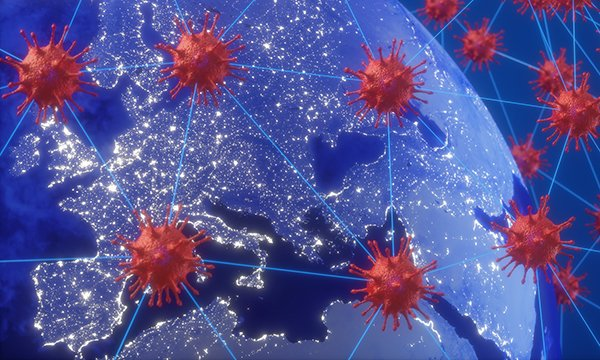
\includegraphics[angle=0, width=3.8cm]{Covid19.png}}
                        %\label{Figure 1}
                    \end{figure}
                \end{column}
                  \begin{column}{0.70\textwidth} % Left column width
                    Эпидемии, такие как COVID-19, оказывают серьезное влияние на здоровье населения и экономику. По данным Всемирной организации здравоохранения (ВОЗ), на 2022 год количество заболевших COVID-19 превышает 400 миллионов человек по всему миру, а число смертей от заболевания превышает 5 миллионов. Пандемия также привела к ограничению движения и закрытию многих предприятий, что вызвало экономические проблемы. 
                \end{column}
            \end{columns}

            \medskip
            Математическое моделирование играет важную роль в понимании и контроле инфекционных заболеваний, таких как COVID-19. Оно помогает ученым разрабатывать эффективные стратегии контроля и прогнозировать \\ будущие тенденции.

            % Эпидемии, такие как COVID-19, оказывают серьезное влияние на здоровье населения и экономику. По данным Всемирной организации здравоохранения (ВОЗ), на 2022 год количество заболевших COVID-19 превышает 400 миллионов человек по всему миру, а число смертей от заболевания превышает 5 миллионов. Пандемия также привела к ограничению движения и закрытию многих предприятий, что вызвало экономические проблемы.\newline

            % Математическое моделирование играет важную роль в понимании и контроле инфекционных заболеваний, таких как COVID-19. Оно помогает ученым разрабатывать эффективные стратегии контроля и прогнозировать \\ будущие тенденции.

            % \begin{center}
            %     \emph{This was a labor of love, I hope you like it!}
            % \end{center}
\end{frame}



%* SECTION-2
%------------------------------------------------
% \section{Агентно-ориентированное моделирование распространения эпидемий}
\section{Агентно-ориентированное моделирование}

%------------------------------------------------
\begin{frame}
    \frametitle{Детерминированные модели}
    \fontsize{8}{10}\selectfont{}
     
    Aгент-ориентированное моделирование являются одним из наиболее распространенных методов моделирования в эпидемиологии. Их развитие началось в середине 20-го века и продолжается по сей день. Большая часть научных статей по моделирование эпидемии основан на модели SIR ("Susceptible-Infected-Recovered") и различные её модификации. Модель SIRS является расширением модели SIR.
    \medskip

    \begin{columns}[c]
        \begin{column}{0.5\textwidth}
            \begin{itemize}
                \item \textbf{Уравнение детерминистическая модель SIRS}
            \end{itemize}    
        \end{column}

        \begin{column}{0.5\textwidth}
            \begin{figure}
                \centering
                \vspace{-0.6cm}
                %\caption{Hawkins et al, 2015}
                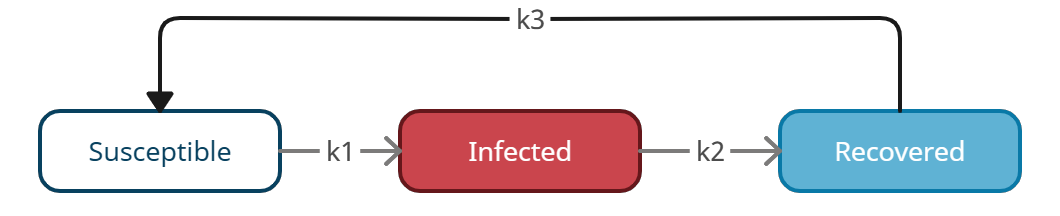
\includegraphics[angle=0, width=4cm]{SIRS.png}
                %\label{Figure 1}
            \end{figure}
        \end{column}
    \end{columns}
 
    \vspace{-0.25cm}
    \begin{columns}[c] % The "c" option specifies centered vertical alignment while the "t" option is used for top vertical alignment
        \begin{column}{0.05\textwidth}
        \end{column}
        \begin{column}{0.25\textwidth}
            \renewcommand{\arraystretch}{1.5}
            \hspace*{\fill}
            $$
            \left\{
            \begin{array}{l}
                \dfrac{d \theta_{\mathit{I}}}{d t}=k_{1} \theta_{\mathit{I}} \theta_{\mathit{S}}-k_{2} \theta_{\mathit{I}} \\[6pt]
                \dfrac{d \theta_{\mathit{R}}}{d t}=k_{2} \theta_{\mathit{I}}-k_{3} \theta_{\mathit{R}} \\
                \theta_{\mathit{S}}+\theta_{\mathit{I}}+\theta_{\mathit{R}}=1
            \end{array}
            \right.
            $$
            \hspace*{\fill}
        \end{column}
        \begin{column}{0.7\textwidth}
            $\theta_{\mathit{S}}$ - концентрация восприимчивых людей (которые могут заразиться)\\
            $\theta_{\mathit{I}}$ - x - концентрация инфицированных \\
            $\theta_{\mathit{R}}$ - концентрация выздоровевших и имеющих иммунитет.\\
            Рассматривается задача Коши с начальными условиями $\theta_{\mathit{I}}(0)$, $\theta_{\mathit{R}}(0)$. \\
            $k_1$ – скорость заражения, $k_2$ – скорость выздоровления, $k_3$ – скорость потери иммунитета $[ед.вр.^{-1}]$. Смертность не учитывается.
        \end{column}
	\end{columns}

    \vspace{-0.25cm}
    \begin{itemize}
        \item \textbf{Преимущество} детерминистической модели SIRS - ее точности и  простота использования.
        \item \textbf{Недостаток} - в упрощенном подходе к описанию распространения инфекции.
    \end{itemize} 


\end{frame}

%------------------------------------------------
\begin{frame}
	\frametitle{Решёточная агентно-ориентированная модель SIRS}
    \fontsize{8}{10}\selectfont{}

    \begin{block}{\small Наша задача}
        Исследование более сложных и контекстуализированных \textbf{стохастических моделей} пространственной эпидемиологии, основанные на динамике пространственной эпидемиологии. Рассмотрим местоположение инфицированных и восприимчивых популяций, а также взаимодействия между ними, а также подвижность (миграция) населения в модели.
    \end{block}

    \begin{itemize}
        \item \textbf{Решёточная агентно-ориентированная модель распространения эпидемий SIRS}
    \end{itemize}

    \begin{columns}[t] % The "c" option specifies centered vertical alignment while the "t" option is used for top vertical alignment
        \begin{column}{0.02\textwidth}
        \end{column}

        \begin{column}{0.38\textwidth}
            \fontsize{6}{4}\selectfont{Решёточная агентно-ориентированная модель 18 \times 18}

            \begin{figure}
                \vspace{-0.1cm}
                \centering
                % \vspace{-0.6cm}
                %\caption{Hawkins et al, 2015}
                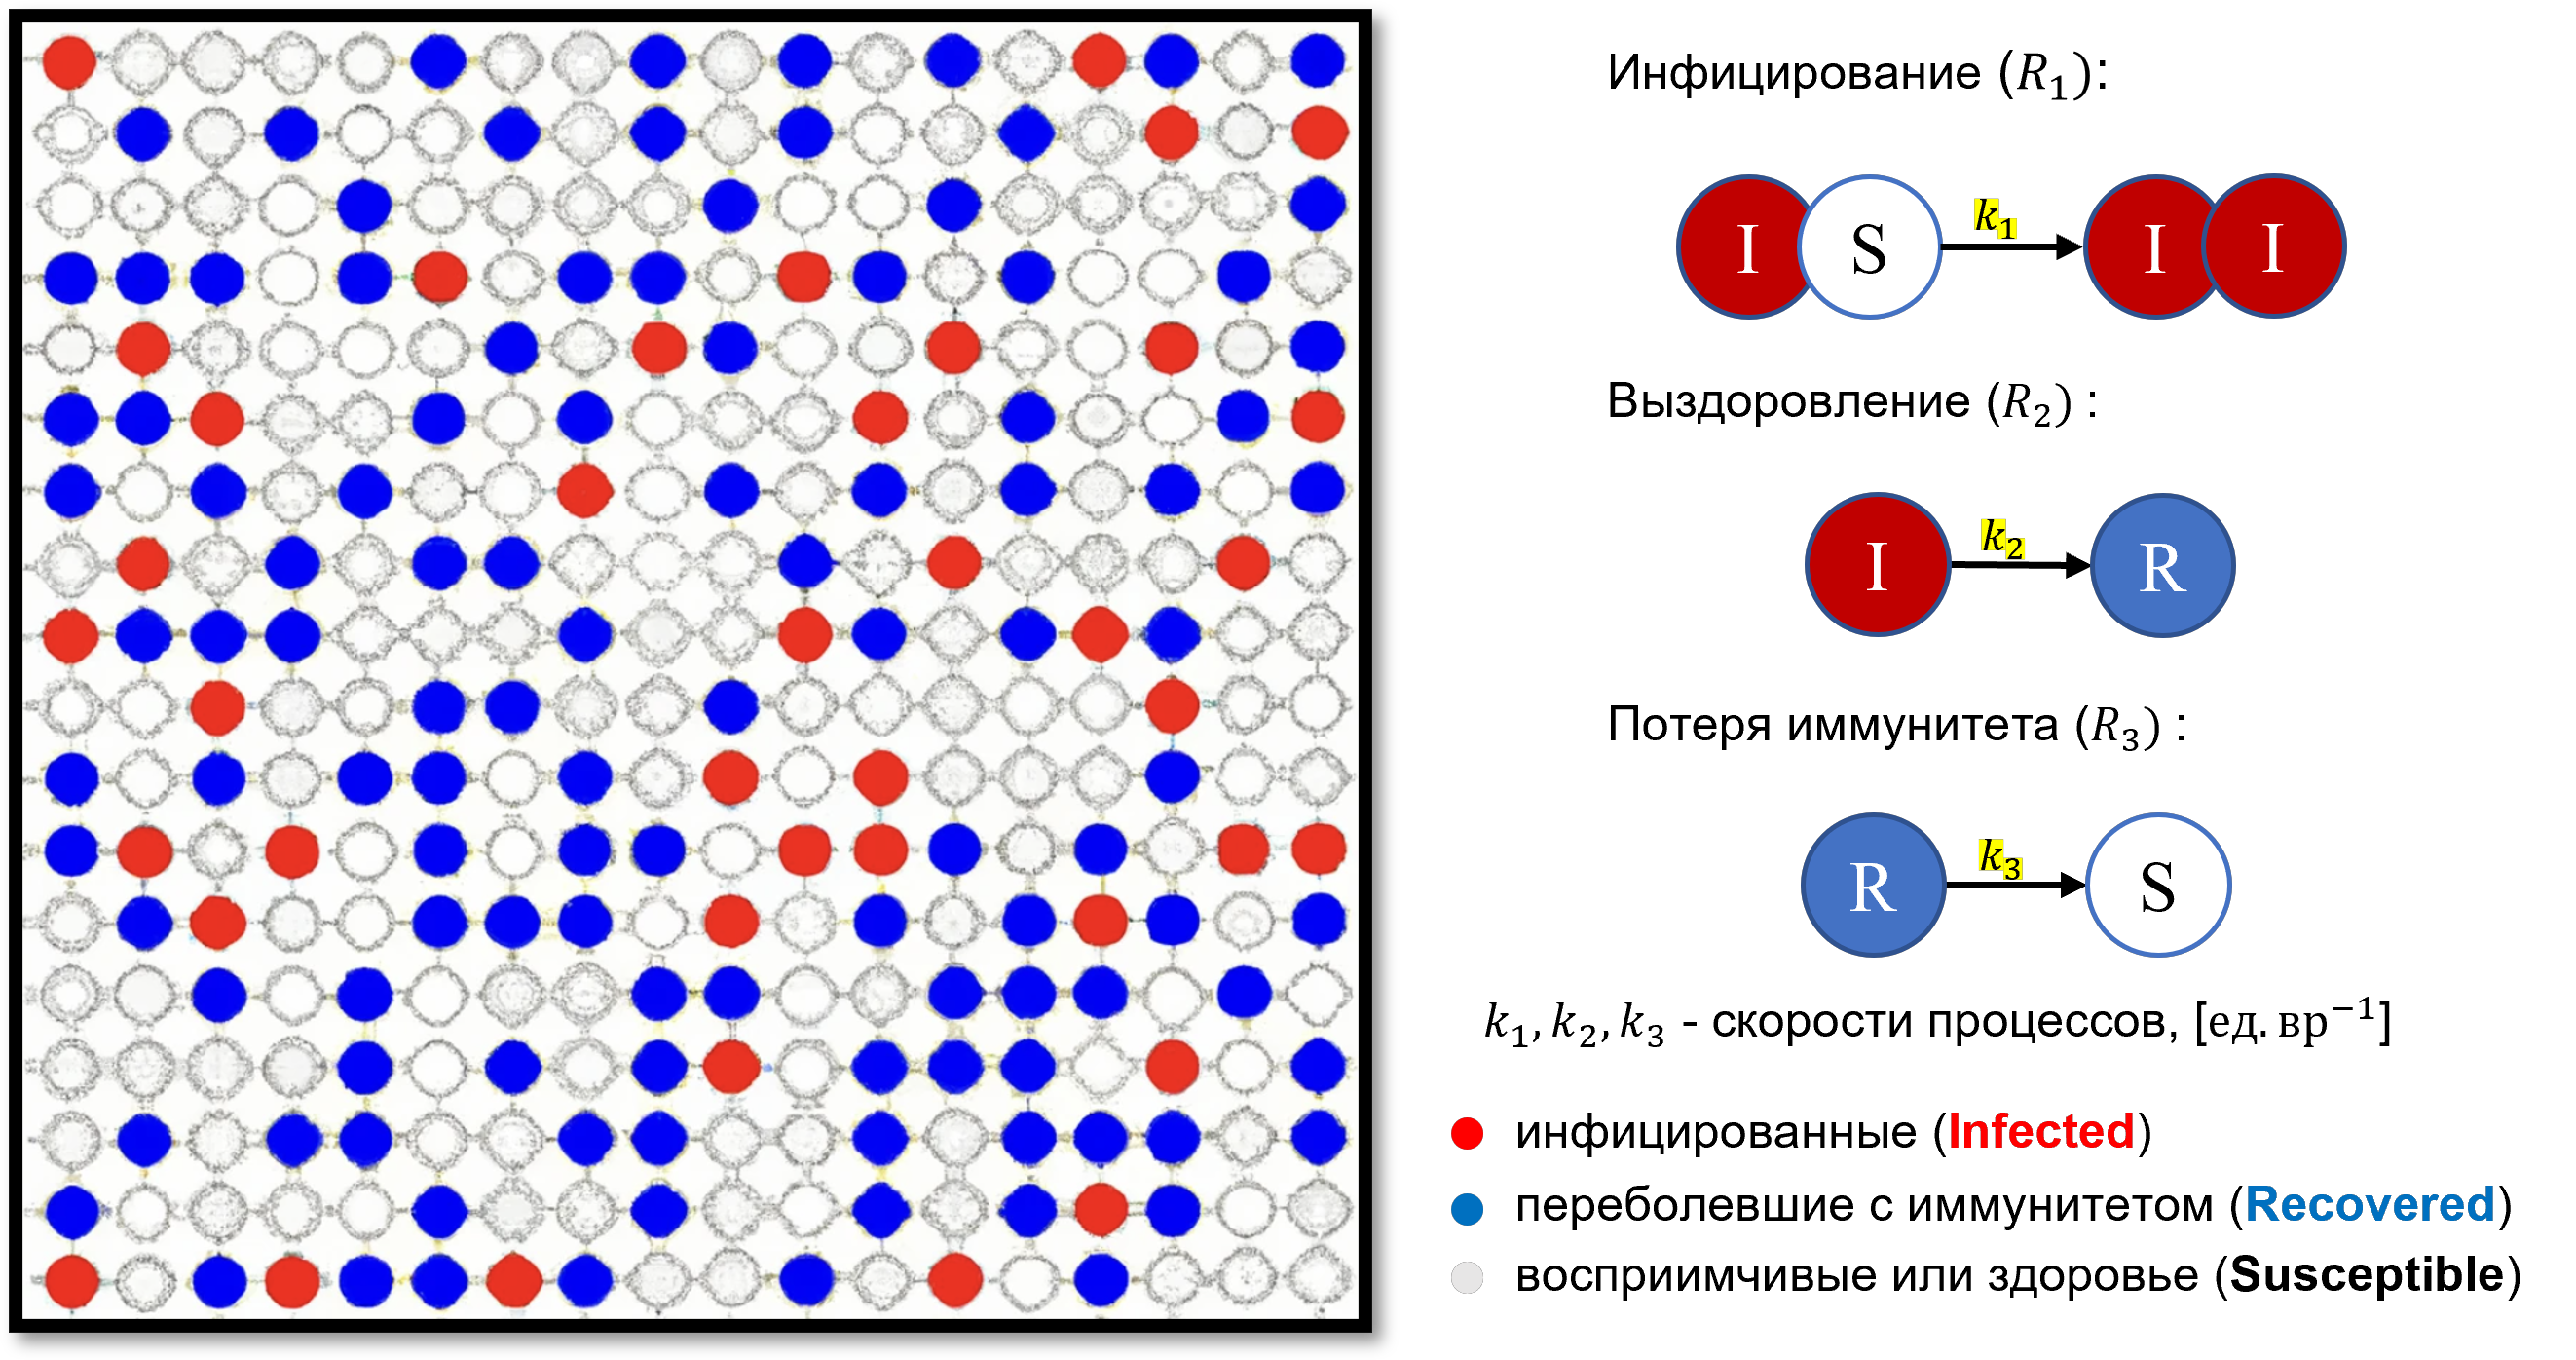
\includegraphics[angle=0, width=6cm]{Grid.png}
                %\label{Figure 1} 
            \end{figure}
        \end{column}

        % \vspace{-1cm}
        \begin{column}{0.6\textwidth}
            Индивидуумы в модели могут находиться на узлах регулярной решетки или на связях в сети на графе. \\
            Три возможных состояния узлов (индивидуумов) в решеточной агентно-ориентированной модели SIRS включают инфицированных (\textcolor{red}{\textbf{Infected}}), переболевших с иммунитетом (\textcolor{blue}{\textbf{Recovered}}) и восприимчивых (\textbf{Suspectable}). Каждое состояние соответствует различным стадиям инфекционного процесса. \\
            Инфицированные узлы могут передавать инфекцию восприимчивым узлам, а переболевшие с иммунитетом узлы могут иметь защиту от повторной инфекции.
        \end{column}
	\end{columns}

\end{frame}

%* SECTION-3
%------------------------------------------------
% \section{Применение кинетического метода Монте-Карло}
\section{Стохастическое моделирование}

%------------------------------------------------
\begin{frame}
	\frametitle{Расширение кинетическая схема модели}
    \fontsize{8}{10}\selectfont{}

    При стохастическом моделировании рассматривается расширенная кинетическая схема модели SIRS, которая включает также и процессы миграции, то есть перемещения индивидуумов по узлам решетки:

    \vspace{-0.2cm}

    \begin{columns}[t] % The "c" option specifies centered vertical alignment while the "t" option is used for top vertical alignment
        \begin{column}{0.02\textwidth}
        \end{column}

        \begin{column}{0.38\textwidth}
            \begin{align*}
                (1) \quad& I_{i}+S_{j} \stackrel{k_{1}}{\rightarrow} I_{i}+I_{j}  &&( \text{инфицирование}  ) \\
                (2) \quad& I_{i} \stackrel{k_{2}}{\rightarrow} R_{i}   &&(\text{выздоровление} ) \\
                (3) \quad& R_{i} \stackrel{k_{3}}{\rightarrow} S_{i} \quad \text{(SIRS)}  &&( \text{потеря иммунитета} ) \\
                (4) \quad& I_{i}+S_{j} \stackrel{d_{1}}{\rightarrow} S_{i}+I_{j}   &&(\text{миграция №1}  ) \\
                (5) \quad& R_{i}+S_{j} \stackrel{d_{2}}{\rightarrow} S_{i}+R_{j}   &&(\text{миграция №2}  ) \\
            \end{align*}
        \end{column}

        \begin{column}{0.28\textwidth}
            \begin{figure}
                \vspace{-0.1cm}
                \hspace{-0.3cm}
                \centering
                % \vspace{-0.6cm}
                %\caption{Hawkins et al, 2015}
                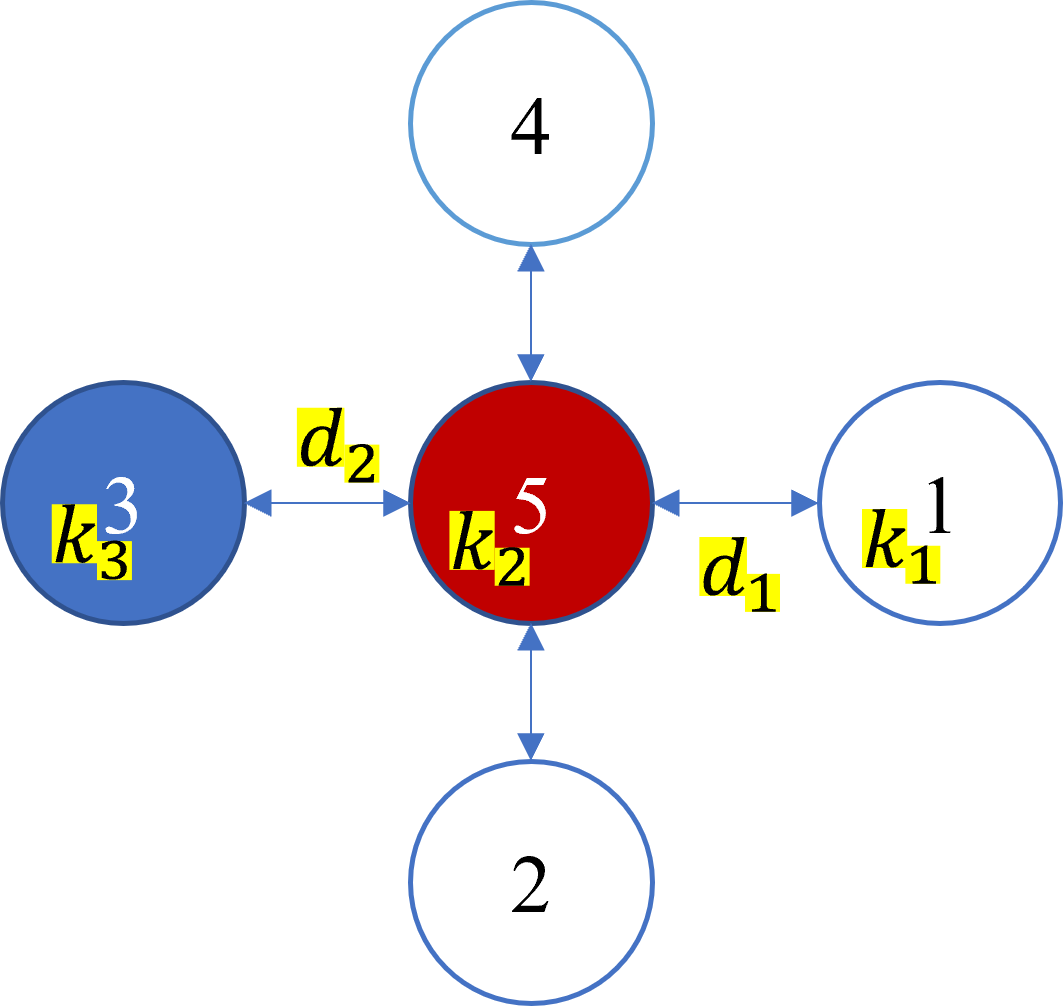
\includegraphics[angle=0, width=3.2cm]{KineticPrinciple-2.png}
                %\label{Figure 1} 
            \end{figure}
        \end{column}

        % \vspace{-1cm}
        \begin{column}{0.3\textwidth}
            \begin{figure}
                \vspace{-0.1cm}
                \centering
                % \vspace{-0.6cm}
                %\caption{Hawkins et al, 2015}
                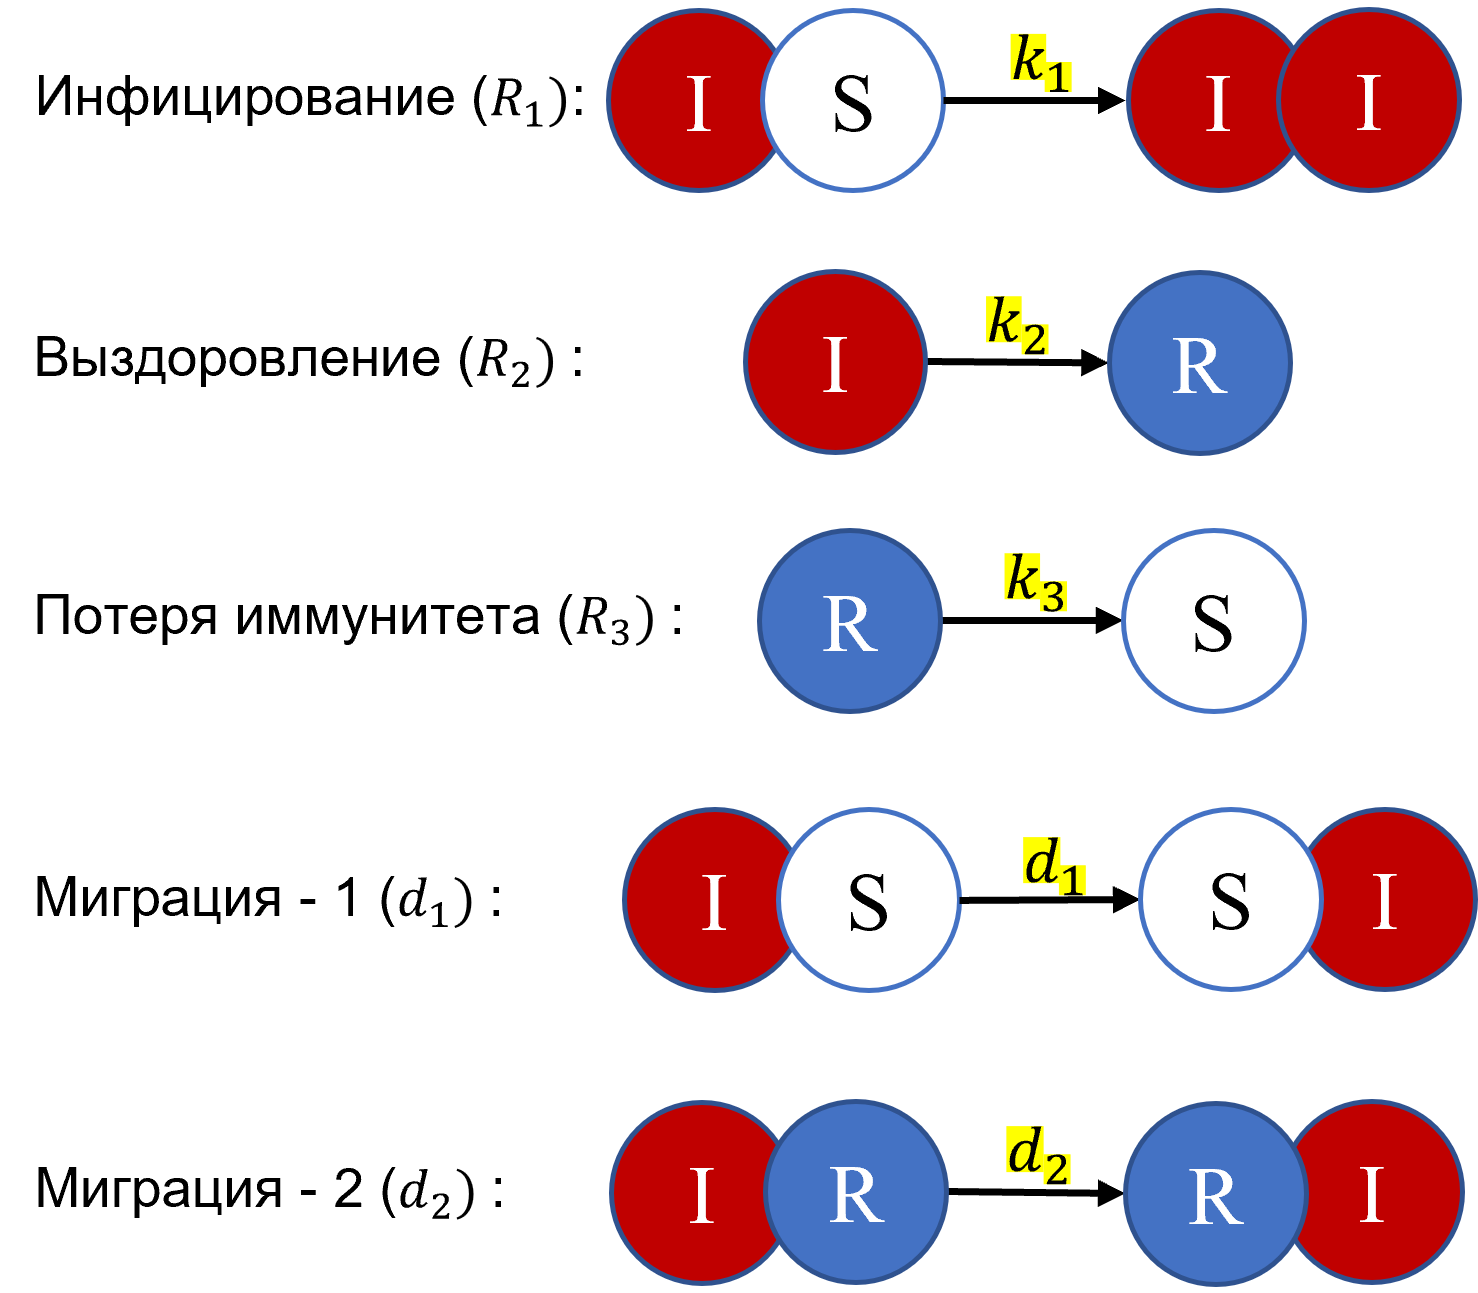
\includegraphics[angle=0, width=3.5cm]{KineticPrinciple.png}
                %\label{Figure 1} 
            \end{figure}
        \end{column}

        \begin{column}{0.02\textwidth}
        \end{column}
	\end{columns}

    \vspace{-0.2cm}

    Рассмотрим микромодель с пятью возможными элементарными событиями, происходящими с интенсивностями $k1$, $k2$, $k3$, $d = d_1 = d_2$. В модели учитывается ограниченное число контактов между людьми, используя пространственную решётку и процесс миграции индивидуумов. \\
    Параметр d определяет скорость перемешивания в популяции и учитывает различные ограничительные факторы. Случай $d=0$ соответствует строгим карантинным мерам, а $d \rightarrow \infty$ приближается к макромодели SIRS с полным перемешиванием, которое на практике невозможно.

\end{frame}

%------------------------------------------------
\begin{frame}
    \frametitle{Марковский стохастический процесс}
		
    \fontsize{8}{10}\selectfont{}

    \vspace{-0.2cm}
    \begin{itemize}
        \item \textbf{Марковский стохастический процесс}
    \end{itemize}

    В решеточной агентно-ориентированной модели SIRS, эволюция системы описывается марковским случайным процессом с дискретным множеством состояний и непрерывным временем. Потоки событий являются независимыми пуассоновскими потоками с заданными интенсивностями. При предположении случайного перемешивания, можем описать изменение вероятностей наблюдения всех возможных дискретных состояний решетки во времени с помощью основного кинетического уравнения (ОКУ, "master equation"):

    \vspace{-0.2cm}

    $$
    \frac{d \mathrm{P}_{i}(t)}{d t}=\sum_{j \neq i}\left(\mathrm{P}_{j}(t) \lambda_{j i}(t)-\mathrm{P}_{i}(t) \lambda_{i j}(t)\right), \quad i=1,2, \ldots, N_{e q}=3^{N} \\
    $$

    \vspace{-0.8cm}

    в уравнении, $\mathrm{P}_{i}$ - вероятность состояния решетки с номером  i , $\lambda_{i j}$ и $\lambda_{j i}$ - скорость перехода из состояния $i$ в состояние $j$  [$ед. вр.^{-1}$] и наоборот.\\
    Для решёточной микромодели SIR/SIRS ОКУ содержит $3^N$ линейных ОДУ первого порядка. Решать такую систему \textbf{невозможно} даже при использовании маленьких решёток, например, для решётки размеров $10 \times 10$ система уже содержит приблизительно $5.2 \times 10^{47}$ уравнений.

    \begin{itemize}
        \item  Одно из решений заключается в том, что мы можем рассчитать отдельные траектории эволюции система, используч \textbf{кинетический метод Монте-Карло} ("Kinetic Monte Carlo", KMC).
    \end{itemize}
   
    % Существует несколько статистически эквивалентных вариантов реализации метода KMС. Один из таких вариантов называется \textbf{прямым методом} (“direct method”) и относится к варианту алгоритмов “без отказов” (“rejection-free”).

\end{frame}

%------------------------------------------------
\logo{}
\begin{frame}
    \frametitle{Кинетический метод Монте-Карло (KMC)}
		
    \fontsize{8}{10}\selectfont{}

    \vspace{-0.2cm}

    \begin{block}{\fontsize{8}{10}\selectfont{Прямой метод КМС (aлгоритм “без отказов”, алгоритм Гиллеспи для решёточной модели)}}
        Кинетический метод Монте-Карло ("без отказов") - это вычислительный подход для моделирования стохастических систем, основанный на случайном выборе событий и изменении состояний системы. "Без отказов" означает учет всех возможных событий сразу, без повторного выбора.
    \end{block}

    \begin{columns}[t] % The "c" option specifies centered vertical alignment while the "t" option is used for top vertical alignment
        % \begin{column}{0.05\textwidth}
        % \end{column}
        \begin{column}{0.75\textwidth}
                \textit{\textbf{Этап №1.} Задание начального состояния решётки.} \\
                \textit{\textbf{Этап №2.}Вычисление скоростей элементарных событий.} На момент $t_1$ вычисляются скорости всех элементарных событий, обновляющих решётку, и определяется суммарная скорость $R$. \\
                \textit{\textbf{Этап №3.}Выбор события и изменение состояния решётки.} Случайно выбирается элементарное событие с вероятностью, пропорциональной его скорости, и изменяется состояние решётки соответственно, и $\sum_{j=1}^{p-1} v_{j}<\xi_{2} V \leq \sum_{j=1}^{p} v_{j}$.\\
                \textit{\textbf{Этап №4.}Вычисление шага по времени. } Вычисляется момент времени   выхода системы из текущего состояния: $t_2 = t_1 - (ln(\xi) / R)$, где  $\xi$  - случайная величина, равномерно распределённая на интервале $(0, 1)$. \\
                \textit{\textbf{Этап №5.}Проверка критерия окончания моделирования.} Осуществляется переход на следующий шаг к этапу II, если не достигнуто заданное максимальное значение времени. \\
        \end{column}

        \begin{column}{0.25\textwidth}
            \begin{figure}
                \vspace{-0.5cm}
                \hspace{-0.3cm}
                % \centering
                %\caption{Hawkins et al, 2015}
                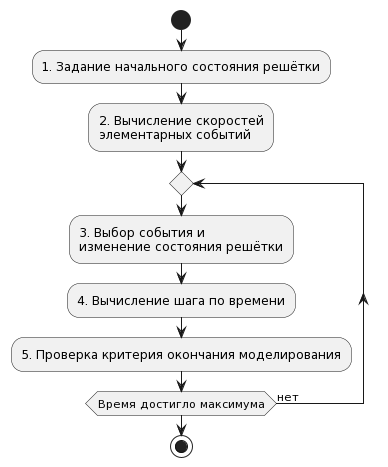
\includegraphics[angle=0, width=3.5cm]{Algorithm.png}
                %\label{Figure 1} 
            \end{figure}
        \end{column}
	\end{columns}

\end{frame}

%* SECTION-4
%------------------------------------------------
\logo{
\includegraphics[width=0.5cm]{logo_vmk_so_shriftom.png}}
\section{Заключение}
%------------------------------------------------
\begin{frame}
	\frametitle{\fontsize{8}{10}\selectfont{Сравнение результатов вычислений детерминированных и стохастических моделей при одинаковых параметрах}}
		
	Last bit of text

\end{frame}

%------------------------------------------------
\begin{frame}
	\frametitle{\fontsize{8}{10}\selectfont{Сравнение результатов моделирования стохастической модели при различных скоростях диффузии}}
		
	Last bit of text

\end{frame}

%------------------------------------------------
\begin{frame}
	\frametitle{\fontsize{8}{10}\selectfont{Моделирование и анализ пространственных эпидемий на больших решетках}}
		
	Last bit of text

\end{frame}

%------------------------------------------------
\begin{frame}
	\frametitle{\fontsize{8}{10}\selectfont{Заключение и планы для дальнейших исследований}}
		
	Last bit of text

\end{frame}

%---------------------------------------------------------
%	CLOSING SLIDE
%---------------------------------------------------------

% To remove miniframe from top
\appendix
\setbeamertemplate{headline}{}
\addtobeamertemplate{frametitle}{\vspace*{-\headheight}}{}

\begin{frame}[noframenumbering] %So the end and appendix slides don't contribute to the page count
%[plain] % The optional argument 'plain' hides the headline and footline
	%\frametitle{Questions?}

	\begin{center}
            {\LARGE Спасибо за внимание!}
	\end{center}
 
\end{frame}

%---------------------------------------------------------
%	REFERENCES
%---------------------------------------------------------

\begin{frame}[noframenumbering, allowframebreaks]
%---------------------------------------------------------

    \frametitle{References}
    \printbibliography

\end{frame}

\begin{frame}
%---------------------------------------------------------
	\frametitle{Список литературы}
		
    \fontsize{10}{10}\selectfont{}

    \begin{enumerate}
        \item \textit{Мюррей \,Дж.}, Математическая биология. Том 1: Введение. – М.: Ижевск: Регулярная и хаотическая динамика: Ин-т компьютерных исслед., 2009, с.\,1104. Том 2: Пространственные модели и их приложения в биомедицине. – М.: Ижевск: Регулярная и хаотическая динамика: Ин-т компьютерных исслед., 2011, с.\,1104.
        \item \textit{De Souza \,D.\,R., Tomé \,T.}, Stochastic lattice gas model describing the dynamics of the SIRS epidemic process // Physica A, 2010, Vol.\,389, P.\,1142–1150.
        \item  \textit{Chatterjee\,A., Vlachos\,D.\,G.}, An overview of spatial microscopic and accelerated kinetic Monte Carlo methods // J. Computer-Aided Mater Des., 2007, Vol.\,14., P.\,253–308.
        \item \textit{Gillespie\,D.\,T.}, A general method for numerically simulating the stochastic time evolution of coupled chemical reactions // J.\,Comput.\,Phys., 1976, Vol.\,22, P.\,403–434.
        \item \textit{A.\,B.\,Bortz, M.\,H.\,Kalos, J.\,L.\,Lebowitz.}, A new algorithm for Monte Carlo simulation of Ising spin systems // J.\,Comp.\,Phys., 1975, Vol.\,17, P.\,10-18.
    \end{enumerate}
 
\end{frame}

\end{document} 